\begin{figure}[tbp]
\centering
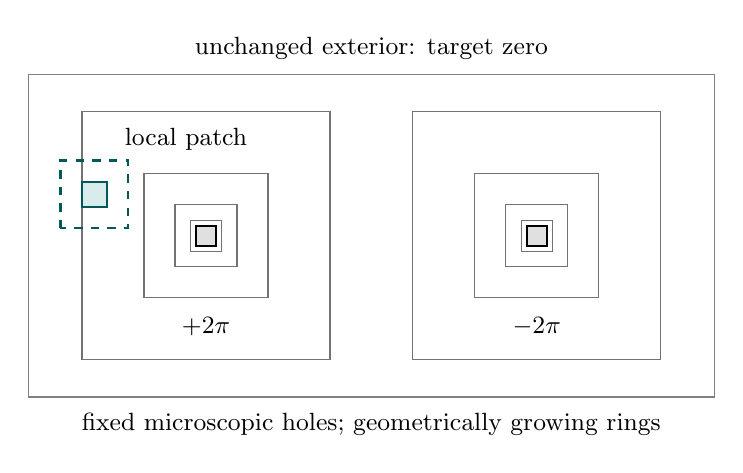
\begin{tikzpicture}[x=1.05cm,y=1.05cm,font=\small]
 \draw[black!50] (-4.15,-1.95) rectangle (4.15,1.95);
 \foreach \x in {-2,2} {
  \foreach \r in {1.5,.75,.375,.1875}
   {\draw[black!55] (\x-\r,-\r) rectangle (\x+\r,\r);}
  \fill[black!12] (\x-.12,-.12) rectangle (\x+.12,.12);
  \draw[thick] (\x-.12,-.12) rectangle (\x+.12,.12);
 }
 \filldraw[fill=teal!15,draw=teal!70!black,thick]
  (-3.5,.35) rectangle (-3.2,.65);
 \draw[teal!70!black,dashed,thick]
  (-3.76,.09) rectangle (-2.94,.91);
 \node[above right] at (-3.1,.91) {local patch};
 \node[fill=white,inner sep=1pt] at (-2,-1.1) {$+2\pi$};
 \node[fill=white,inner sep=1pt] at (2,-1.1) {$-2\pi$};
 \node[above] at (0,2.02) {unchanged exterior: target zero};
 \node[below] at (0,-2.03)
  {fixed microscopic holes; geometrically growing rings};
\end{tikzpicture}
\caption{Schematic geometry for the winding-sector comparison.
Each square ring is partitioned into tiles much smaller than its
distance to the source; only one tile and its enlarged patch are
shown. The construction trims tile junctions and uses collars
with full interfaces. The number of processed tiles is
\(O_M(1+\log n)\), while the unprocessed exterior is kept intact.}
\label{fig:annuli}
\end{figure}
